\documentclass[a4paper]{article}

\usepackage{graphicx}
\usepackage{amsmath,amssymb}
\usepackage{minted}
\usepackage{multirow}
\usepackage{float}
\usepackage{algorithm}
\usepackage{algpseudocode}
\usepackage{todonotes}
\usepackage{forest}
\usepackage{xstring}
\usepackage{xcolor}
\usepackage[most]{tcolorbox}
\usepackage{xparse}
\usepackage{natbib}
\usepackage{adjustbox}

\usetikzlibrary{graphs,graphdrawing}
\usegdlibrary{layered}

% for external graphviz
\input{/home/donkarlo/Dropbox/repo/nd_language_ai_project/src/nd_language_ai/formal/computer/programming/tex/latex/code_clips/external_graphviz.tex}

% for tags
\input{/home/donkarlo/Dropbox/repo/nd_language_ai_project/src/nd_language_ai/formal/computer/programming/tex/latex/part/control_sequence/kind/semtag/semtag.tex}

% for links
\input{/home/donkarlo/Dropbox/repo/nd_language_ai_project/src/nd_language_ai/formal/computer/programming/tex/latex/code_clips/seehere.tex}

% for nested lists and sections
\input{/home/donkarlo/Dropbox/repo/nd_language_ai_project/src/nd_language_ai/formal/computer/programming/tex/latex/code_clips/deep_structure.tex}

\title{Code implementation}
\date{}
\author{Mohammad Rahmani}

\begin{document}
   \maketitle
   \section{Modules}
      \subsection{nd\_social\_mind}

         \seeherefooter{https://github.com/donkarlo/nd\_sociomind\_project}


      \subsection{nd\_robotic\_ai}

         \seeherefooter{https://github.com/donkarlo/nd\_robotic\_ai\_project}


      \subsection{nd\_math}

         \seeherefooter{https://github.com/donkarlo/nd\_math\_project}


      \subsection{nd\_datascience}

         \seeherefooter{https://github.com/donkarlo/nd\_datascience\_project}


      \subsection{nd\_physics}

         \seeherefooter{https://github.com/donkarlo/nd\_physics\_project}


      \subsection{nd\_utility}

         \seeherefooter{https://github.com/donkarlo/nd\_utility\_project}
      \subsection{Module relations}
         \begin{figure}[H]
            \centering
            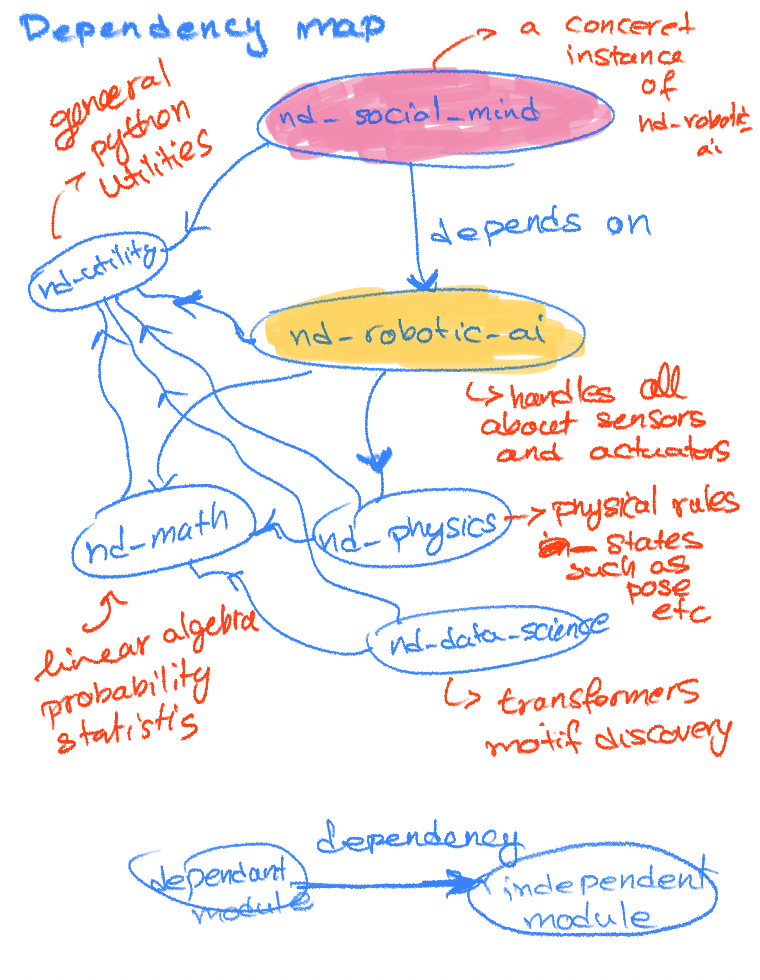
\includegraphics[width=0.9\textwidth]{modules_relation.png}
         \end{figure}
   \section{Robot composition}
      Using the same onthology described in methodology. That is composition design pattern is used to build a  robot.
      \subsection{Quadcopter}
         For example a quadcodcopter is composed of
         \begin{figure}[H]
            \centering
            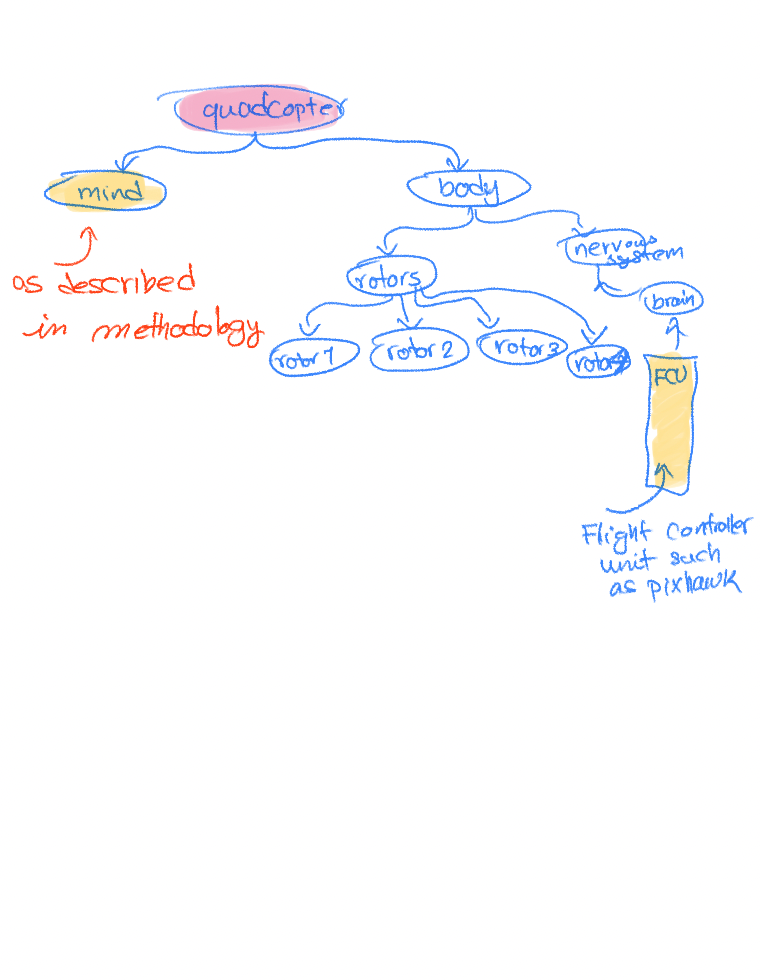
\includegraphics[width=0.9\textwidth]{quadcopter.png}
         \end{figure}
   \section{Multi robot system}
      Multi robot system is also implemented using composition design pattern. Such that each group can have subgroups. For example in this research two drnoes which were guided by a human agent is implemented as show in Figure ~\ref{multi_robot_system_code}
      Each group must have a relationship whic inforces the laws of that relationship. As soon as a robot is defined ina group, a role must be assigned to it.
      \begin{figure}[H]
         \centering
         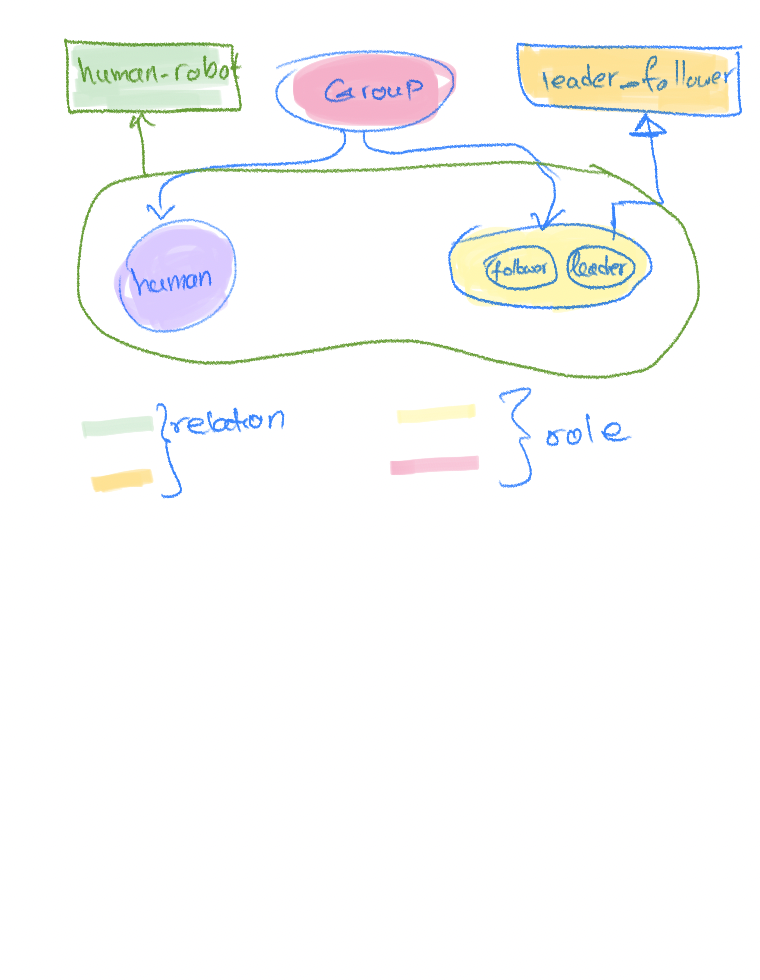
\includegraphics[width=0.9\textwidth]{multi_robot_system_code.png}
         \label{multi_robot_system_code}
      \end{figure}

      \bibliographystyle{plainnat}
      \bibliography{/home/donkarlo/Dropbox/repo/nd_shared_research/bibliography/bibliography.bib}
\end{document}
